% ================== Kapitel: Methoden ============================================

\section{Vorgehen und gewünschte Methoden}
In diesem Abschnitt wird kurz beschrieben, welche Vorgehensweise und Methoden
bereits vor Projektstart gemeinsam mit dem Auftraggeber festgelegt wurden.
Die Aufgabenstellung sah ein inkrementelles, iteratives und agiles Vorgehen vor
(siehe die Aufgabenstellung unter Abschnitt~\ref{sec:aufgabenstellung}). 
Dieses Vorgehen wurde zu Beginn des Projekts gemeinsam besprochen und als 
passend für den Projektumfang eingeschätzt.

Konkret wurde vereinbart, alle zwei Wochen ein Meeting mit dem Auftraggeber
durchzuführen. In diesen Meetings wurde jeweils der aktuelle Projektstand
vorgestellt, offene Punkte und Risiken besprochen sowie das weitere Vorgehen
abgestimmt. Zusätzlich sollte der Projektfortschritt jederzeit transparent
nachvollziehbar sein. Dafür wurde GitLab als zentrales Tool zur Aufgabenverwaltung
verwendet, in dem der aktuelle Stand laufend gepflegt wurde. Dieses Vorgehen
hat sich über die gesamte Projektdauer bewährt und wurde konsequent umgesetzt.

Die regelmässigen Meetings waren insgesamt sehr hilfreich und konstruktiv.
Durch den engen Austausch konnten Anforderungen frühzeitig überprüft und
bei Bedarf angepasst werden. Auf diese Weise fand bereits während der
Entwicklung eine formale Validierung der Anforderungen statt
(siehe Abschnitt~\ref{sec:anforderung-validierung}).
Alle Sitzungsprotokolle und Statusberichte sind im Anhang dokumentiert
(siehe Anhang~\ref{sec:protokolle-statusberichte}).

\section{Kreativität und Innovation}
Ein weiterer Schwerpunkt des Projekts lag auf dem Einsatz moderner
Technologien und Entwicklungsansätze. Vorgesehen war unter anderem die
Evaluation aktueller Android-Technologien wie Jetpack Compose sowie der
Einsatz von CI/CD-Automatisierungen und AI-gestützten Entwicklungswerkzeugen.

Diese Vorgaben wurden im Projekt aktiv umgesetzt. Die App wurde auf Basis
aktueller Bibliotheken und SDK-Versionen entwickelt, sodass auch moderne
Geräte und neue Android-Versionen unterstützt werden. Die Entwicklung folgte
dabei einem \textit{AI-first}-Ansatz, bei dem KI-Tools gezielt zur Unterstützung
bei Architekturentscheidungen, Code-Erstellung, Refactorings und Dokumentation
eingesetzt wurden. Die Nutzung dieser Werkzeuge wurde laufend reflektiert und
je nach Projektsituation angepasst, um einen sinnvollen Mehrwert für die
Entwicklung zu erzielen (siehe ~\ref{sec:ai-reflexion}).

\section{Domain Driven Design}

Domain Driven Design (DDD) war als Grundlage für die
Projektstruktur vorgegeben. Ziel war es, die fachlichen Domänen der App klar
zu trennen und im Code sauber abzubilden.

Die Anwendung ist in klar abgegrenzte Bereiche unterteilt, wobei gemeinsame
und fachlich unabhängige Komponenten in \texttt{common}-Modulen liegen und
fachspezifische Logik in den jeweiligen \texttt{features}-Modulen umgesetzt
ist. Jedes Feature bildet dabei eine eigene fachliche Domäne ab. 
Diese Struktur war bereits in der bestehenden iOS-Applikation umgesetzt und
wurde für das Android-Projekt bewusst in gleicher Form übernommen.

\section{Projektmanagement}

\subsection{Stakeholder}
\begin{itemize}
    \item Auftraggeber / Dozent: Jürg Nietlispach
    \item Experte: Martin Vogel
    \item Projektteam: Raphael Eiholzer, Samuel Kurmann
\end{itemize}

\subsection{Planung}
Um zu Beginn einen Überblick über das Projektmanagement zu erhalten, wurden
alle bekannten Termine wie Abgaben, Präsentationen und Meilensteine in einer
Excel-Tabelle gesammelt. Diese diente während der gesamten Projektdauer als
eine Art Meilensteinplan und half dabei, den zeitlichen Rahmen des Projekts
übersichtlich darzustellen.

Auf dieser Grundlage konnten die anstehenden Arbeiten sinnvoll in einzelne
Sprints aufgeteilt werden. Die Excel-Übersicht wurde insbesondere zu Beginn
des Projekts genutzt, während die weitere Detailplanung und Aufgabenverwaltung
anschliessend agil über GitLab erfolgte.

\vspace{1.2em}
\begin{figure}[H]
    \centering
    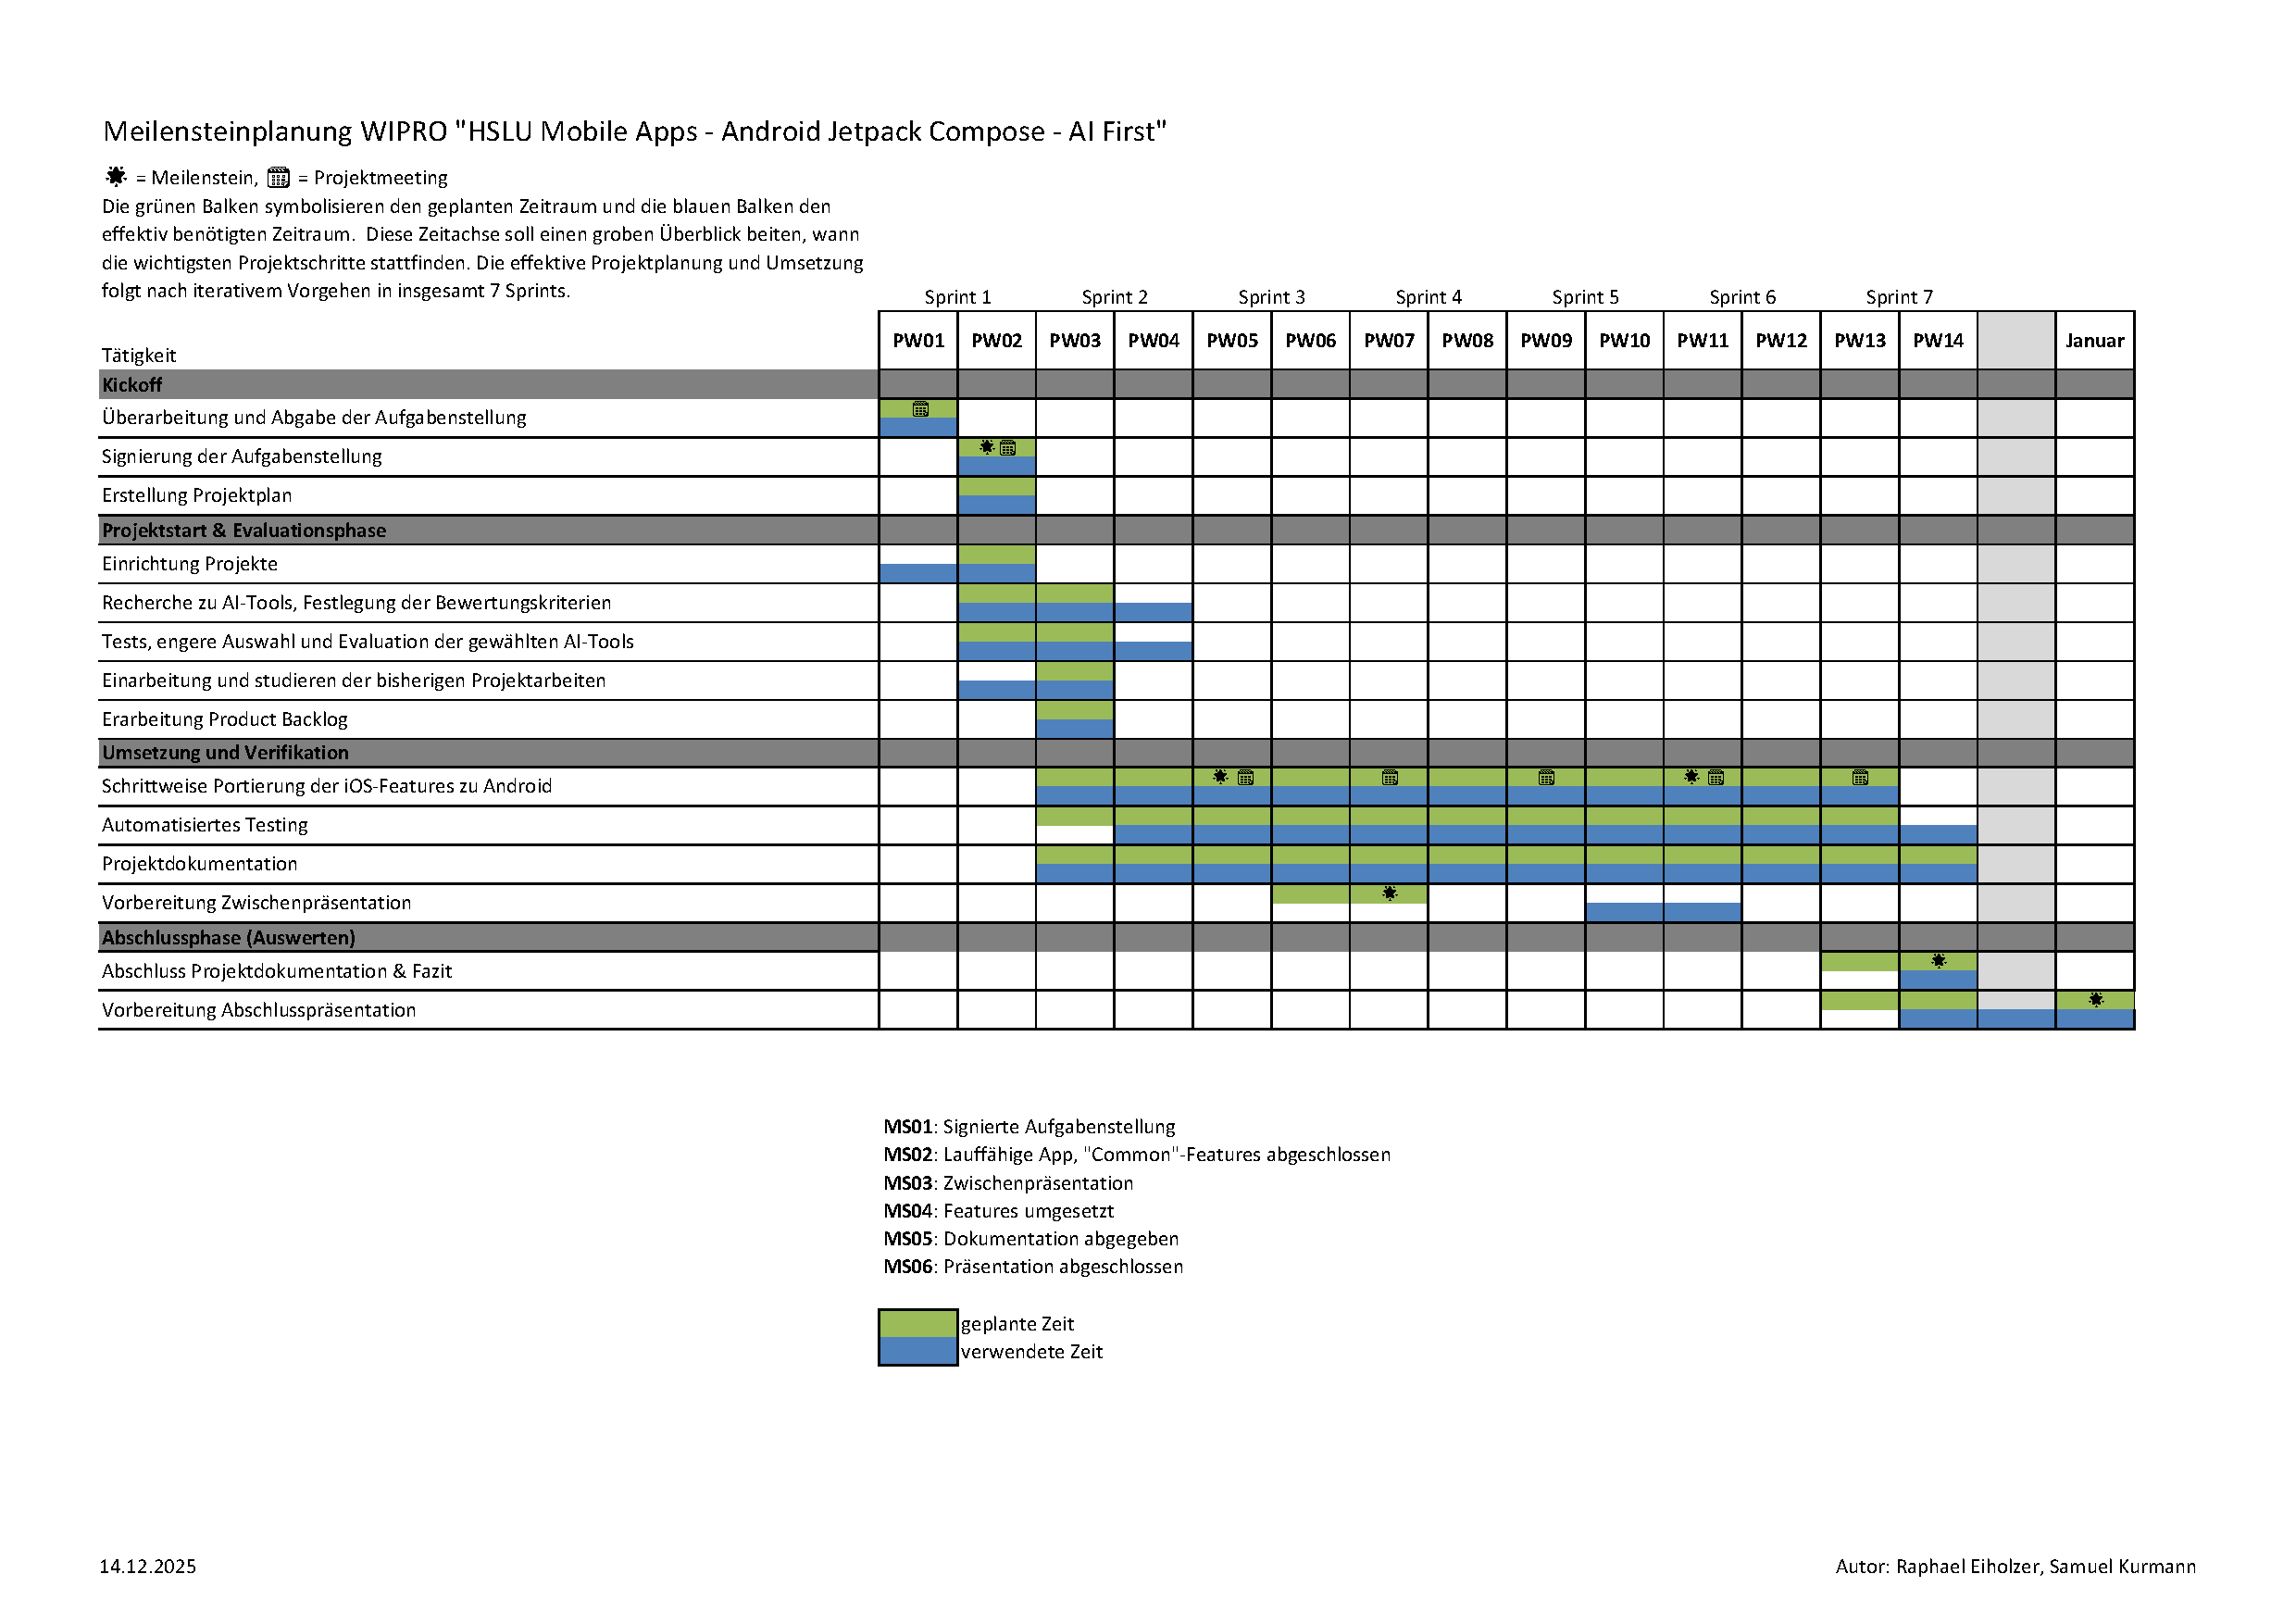
\includegraphics[width=0.85\textwidth]{Fotos/zeitplan.png}
    \caption{Meilensteinplan des Projekts}
    \label{fig:meilensteinplan}
\end{figure}\newpage

\subsection{Agiles Vorgehen}
Die Umsetzung des Projekts erfolgte nach einem agilen Vorgehen, angelehnt an
Scrum. Die Arbeit wurde in zweiwöchige Sprints unterteilt, woraus sich insgesamt
sieben Sprints ergaben. Vor jedem Sprint wurde im Team gemeinsam besprochen,
welche Aufgaben im kommenden Zeitraum umgesetzt werden sollen und wer welche
Arbeiten übernimmt.

\begin{figure}[H]
    \centering
    \includegraphics[width=0.35\textwidth]{Fotos/sprint_cycle.png}
    \caption{Darstellung des Scrum-Prozesses im Projekt} \parencite{atlassian_atlassian_nodate}
    \label{fig:scrum}
\end{figure}

Dieses Vorgehen ermöglichte ein effizientes Arbeiten, da Aufgaben flexibel
verteilt und bei freier Kapazität jederzeit neue Issues übernommen werden
konnten. Da alle Aufgaben und der aktuelle Projektstand in GitLab erfasst
waren, hatte auch der Auftraggeber jederzeit Einblick in den Fortschritt des
Projekts.

Zur Nachvollziehbarkeit des Projektverlaufs sind die Sprint-Backlogs als
grafische Übersicht im Anhang dokumentiert und zeigen den Fortschritt über die
gesamte Projektdauer hinweg (siehe ~\ref{anhang:sprintboard-1}).

\vspace{1.0em}
\begin{figure}[H]
    \centering
    \includegraphics[width=0.99\textwidth]{Fotos/sprintplanung-1.png}
    \caption{Backlogs in GitLab zu Projektbeginn}
    \label{fig:backlog}

\end{figure}\newpage

\subsubsection{Issues}
Alle Aufgaben im Projekt wurden als Issues in GitLab erfasst. Diese wurden
meist als einfache User Stories formuliert und mit einer kurzen
\textit{Definition of Done} (DoD) ergänzt. Dadurch war von Beginn an klar,
was zu einer Aufgabe gehört und wann sie als abgeschlossen gilt. Dies half, 
die Anforderungen besser zu verstehen und Missverständnisse zu
vermeiden.

Für jede Aufgabe wurde die aufgewendete Zeit direkt im jeweiligen Issue
dokumentiert. So konnte der Arbeitsaufwand über die gesamte Projektlaufzeit
hinweg nachvollzogen werden und es war jederzeit ersichtlich, wie viel Zeit
in welche Themen investiert wurde (siehe Anhang~\ref{anhang:zeit}).

\begin{figure}[H]
    \centering
    \includegraphics[width=0.7\textwidth]{Fotos/issue-userstory-dod.png}
    \caption{Beispiel einer User Story mit Definition of Done (DoD)}
    \label{fig:userstory}
\end{figure}

\subsection{Eingesetzte Programme/Tools}
Während der Projektdauer wurden diese Programme und Tools genutzt, um die Entwicklung, 
Dokumentation und die Organisation des Projekts zu unterstützen.

\vspace{0.6em}
\begin{table}[H]
\centering
\begin{tabular}{|l|p{12cm}|}
\hline
\textbf{Werkzeug} & \textbf{Einsatz im Projekt} \\
\hline
Git & Versionsverwaltung des Quellcodes \\
\hline
GitLab & Issue-Tracking, Sprint-Planung und Projektübersicht \\
\hline
OneNote & Persönliche Notizen, Skizzen und Screenshots während der Entwicklung \\
\hline
OneDrive & Zentrale Ablage für Projektdokumente und organisatorische Dateien \\
\hline
Latex & Erstellung und Formatierung der Projektdokumentation \\
\hline
VS Code & Editor zur Erstellung der Dokumentation \\
\hline
GitHub & Hosting des Dokumentations-Quellcodes \\
\hline
Android Studio & Endwicklungsumgebung für die Android-Applikation \\
\hline
Cursor & Endwicklungsumgebung mit AI-Features \\
\hline
Microsoft Teams & Kommunikation im Team und Meetings mit dem Auftraggeber \\
\hline
\end{tabular}
\caption{Eingesetzte Werkzeuge im Projekt}
\label{tab:werkzeuge}
\end{table}\clearpage


\subsection{Risikomanagement}
Zu Beginn des Projekts wurde eine Risikoanalyse erstellt, um die grössten Risiken frühzeitig zu identifizieren und entsprechende Gegenmassnahmen zu planen.  
Die Risiken wurden jeweils hinsichtlich Eintrittswahrscheinlichkeit und Auswirkung bewertet.  
Das Produkt dieser beiden Faktoren bestimmte den Gesamtrisiko-Wert und erlaubte es, die kritischsten Risiken zu priorisieren.  

Für jedes Risiko wurden präventive Massnahmen festgelegt, um die Eintrittswahrscheinlichkeit oder die Auswirkungen zu minimieren.  
Nach Umsetzung dieser Massnahmen wurde die Bewertung erneut vorgenommen, um verbleibende Risiken zu identifizieren und ihre Entwicklung über die Projektlaufzeit zu beobachten.  

\begin{figure}[H]
    \centering
    \includegraphics[width=0.4\textwidth]{Fotos/risikomatrix.png}
    \caption{Risikoanalyse und Risikomatrix des Projekts}
    \label{fig:risikomatrix}
\end{figure}

Die Risikoanalyse wurde während der gesamten Projektdauer regelmässig überprüft und aktualisiert.  
Am Ende jedes Sprints wurde die aktuelle Risikosituation besprochen und mögliche Massnahmen eingeleitet.  
Die drei grössten Risiken wurden zusätzlich an den Auftraggeber übermittelt, um Transparenz über den Projektfortschritt und potenzielle Herausforderungen sicherzustellen.
Die gesamte Risikoanalyse ist im Anhang zu finden (siehe Anhang~\ref{anhang:risk}).